
\documentclass[11pt,oneside]{article} 

\usepackage{a4wide}

\usepackage{amsmath}
\usepackage{color}
%\usepackage{natbib} % kills arxiv 
\usepackage{framed}
%\usepackage{cite}
\usepackage{tikz}
\usepackage{tikz-cd}

% http://www.maths.qmul.ac.uk/~mf/genyoungtabtikz.sty
\usepackage[vcentermath]{genyoungtabtikz}
\Yboxdim{8pt}
%\Ylinethick{1pt}

\RequirePackage{amsmath}
\RequirePackage{amssymb}
\RequirePackage{amsthm}

%\RequirePackage{algorithmic}
%\RequirePackage{algorithm}
%\RequirePackage{theorem}
%\RequirePackage{eucal}
\RequirePackage{color}
\RequirePackage{url}
\RequirePackage{mdwlist}

\RequirePackage{rotating}


\RequirePackage[all]{xy}
%\_CompileMatrices
%\RequirePackage{hyperref}
\RequirePackage{graphicx}
%\RequirePackage[dvips]{geometry}

\usepackage{xcolor}
%\usepackage{amsmath,amsfonts,amssymb}
\usepackage{graphicx}
\usepackage[caption=false]{subfig}
\usepackage{enumerate}
\usepackage{mathrsfs}
\usepackage{bbm}

% -------------- Commands ----------------------

\makeatletter
\newcommand{\verbatimfont}[1]{\renewcommand{\verbatim@font}{\ttfamily#1}}
\makeatother

\newcommand{\Eref}[1]{(\ref{#1})}
\newcommand{\Fref}[1]{Fig.~\ref{#1}}
%\newcommand{\Aref}[1]{Appendix~\ref{#1}}
\newcommand{\SRef}[1]{Section~\ref{#1}}

\newcommand{\todo}[1]{\ \textcolor{red}{\{#1\}}\ }

\newcommand{\Aut}{\mathrm{Aut}}
\newcommand{\Hom}{\mathrm{Hom}}
%\newcommand{\hom}{\mathrm{hom}} % internal hom ?
\newcommand{\Stab}{\mathrm{Stab}}
\newcommand{\Fix}{\mathrm{Fix}}
\newcommand{\Orbit}{\mathrm{Orbit}}
\newcommand{\Ker}{\mathrm{Ker}}
\newcommand{\Image}{\mathrm{Im}}
\newcommand{\Dim}{\mathrm{Dim}}
\newcommand{\Complex}{\mathbb{C}}
\newcommand{\Integer}{\mathbb{Z}}
\newcommand{\Natural}{\mathbb{N}}

\newcommand{\GL}{\mathrm{GL}}
\newcommand{\SL}{\mathrm{SL}}
\newcommand{\SO}{\mathrm{SO}}
\newcommand{\Sp}{\mathrm{Sp}}
\newcommand{\PGL}{\mathrm{PGL}}
\newcommand{\Field}{\mathbb{F}}

% Lemma, proof, theorem, etc.
\newcommand\nounderline[1]{ #1} 
\newcommand\dodef[1]{\vskip 5pt \noindent{\bf \underline{Definition #1.}\ }}
\newcommand\dolemma[1]{\vskip 5pt \noindent{\bf \underline{Lemma #1.}\ }}
\newcommand\doproposition[1]{\vskip 5pt \noindent {\bf \underline{Proposition #1.}\ }}
\newcommand\dotheorem[1]{\vskip 5pt \noindent {\bf \underline{Theorem #1.}\ }}
\newcommand\docorollary[1]{\vskip 5pt \noindent {\bf \underline{Corollary #1.}\ }}
\newcommand\doexample[1]{\vskip 5pt \noindent {\bf \underline{Example #1.}\ }}
\newcommand\doproof{\vskip 5pt \noindent{\bf \nounderline{Proof:}\ }}

\newcommand\tombstone{\rule{.36em}{2ex}\vskip 5pt}

\newcounter{numitem}
\newcommand{\numlabel}[1]{\refstepcounter{numitem}\thenumitem\label{#1}}
\newcommand{\numitem}{\refstepcounter{numitem}\thenumitem}

% Categories
\newcommand{\Set}{\mathbf{Set}}
\newcommand{\FinSet}{\mathbf{FinSet}}
\newcommand{\GSet}{\mathbf{GSet}}
\newcommand{\GRep}{\mathbf{GRep}}
\newcommand{\CRing}{\mathbf{CRing}}

\newcommand{\thinplus}{\!+\!}

\renewcommand{\arraystretch}{1.2}

\newcommand{\tensor}{\otimes}


\newcommand{\DynkinAn}{
  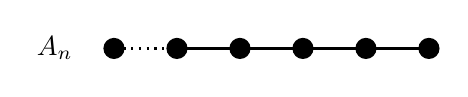
\begin{tikzpicture}[scale=.4]
    \draw (-1,0) node[anchor=east]  {$A_n$};
    \foreach \x in {0,...,5}
    \draw[xshift=\x cm,thick,fill=black] (\x cm,0) circle (.3cm);
    \draw[dotted,thick] (0.3 cm,0) -- +(1.4 cm,0);
    \foreach \y in {1.15,...,4.15}
    \draw[xshift=\y cm,thick] (\y cm,0) -- +(1.4 cm,0);
  \end{tikzpicture}
}

\newcommand{\DynkinAa}{
  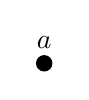
\begin{tikzpicture}[scale=.3]
    \draw (0,0.2) node[anchor=south] {$a$};
    \foreach \x in {0}
    \draw[xshift=\x cm,thick,fill=black] (\x cm,0) circle (.3cm);
  \end{tikzpicture}
}

\newcommand{\DynkinAab}{
  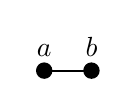
\begin{tikzpicture}[scale=.3]
    \draw (0,0.2) node[anchor=south] {$a$};
    \draw (2,0.2) node[anchor=south] {$b$};
    \foreach \x in {0,1}
    \draw[xshift=\x cm,thick,fill=black] (\x cm,0) circle (.3cm);
    \foreach \y in {0.15,...,0.15}
    \draw[xshift=\y cm,thick] (\y cm,0) -- +(1.4 cm,0);
  \end{tikzpicture}
}

\newcommand{\DynkinAabc}{
  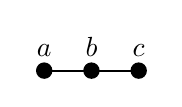
\begin{tikzpicture}[scale=.3]
    \draw (0,0.2) node[anchor=south] {$a$};
    \draw (2,0.2) node[anchor=south] {$b$};
    \draw (4,0.2) node[anchor=south] {$c$};
    \foreach \x in {0,1,2}
    \draw[xshift=\x cm,thick,fill=black] (\x cm,0) circle (.3cm);
    \foreach \y in {0.15,...,1.15}
    \draw[xshift=\y cm,thick] (\y cm,0) -- +(1.4 cm,0);
  \end{tikzpicture}
}

\newcommand{\DynkinAabcd}{
  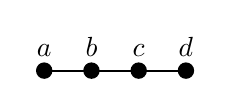
\begin{tikzpicture}[scale=.3]
    \draw (0,0.2) node[anchor=south] {$a$};
    \draw (2,0.2) node[anchor=south] {$b$};
    \draw (4,0.2) node[anchor=south] {$c$};
    \draw (6,0.2) node[anchor=south] {$d$};
    \foreach \x in {0,1,2,3}
    \draw[xshift=\x cm,thick,fill=black] (\x cm,0) circle (.3cm);
    \foreach \y in {0.15,...,2.15}
    \draw[xshift=\y cm,thick] (\y cm,0) -- +(1.4 cm,0);
  \end{tikzpicture}
}


\newcommand{\DynkinBn}{
  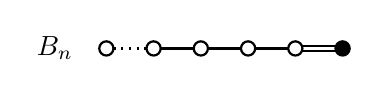
\begin{tikzpicture}[scale=.3]
    \draw (-1,0) node[anchor=east]  {$B_n$};
    \foreach \x in {0,...,4}
    \draw[xshift=\x cm,thick] (\x cm,0) circle (.3cm);
    \draw[xshift=5 cm,thick,fill=black] (5 cm, 0) circle (.3 cm);
    \draw[dotted,thick] (0.3 cm,0) -- +(1.4 cm,0);
    \foreach \y in {1.15,...,3.15}
    \draw[xshift=\y cm,thick] (\y cm,0) -- +(1.4 cm,0);
    \draw[thick] (8.3 cm, .1 cm) -- +(1.4 cm,0);
    \draw[thick] (8.3 cm, -.1 cm) -- +(1.4 cm,0);
  \end{tikzpicture}
}

\newcommand{\DynkinBab}{
  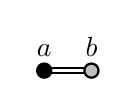
\begin{tikzpicture}[scale=.3]
    \draw (0,0.2) node[anchor=south] {$a$};
    \draw (2,0.2) node[anchor=south] {$b$};
    \foreach \x in {0}
    \draw[xshift=\x cm,thick,fill=black] (\x cm,0) circle (.3cm);
    \foreach \x in {1}
    \draw[xshift=\x cm,thick,fill=lightgray] (\x cm,0) circle (.3cm);
    \foreach \y in {0.15,...,0.15}
    \draw[xshift=\y cm,thick] (\y cm,+0.1 cm) -- +(1.4 cm,0);
    \foreach \y in {0.15,...,0.15}
    \draw[xshift=\y cm,thick] (\y cm,-0.1 cm) -- +(1.4 cm,0);
  \end{tikzpicture}
}

\newcommand{\DynkinBabc}{
  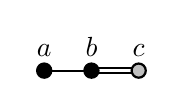
\begin{tikzpicture}[scale=.3]
    \draw (0,0.2) node[anchor=south] {$a$};
    \draw (2,0.2) node[anchor=south] {$b$};
    \draw (4,0.2) node[anchor=south] {$c$};
    \foreach \x in {0,1}
    \draw[xshift=\x cm,thick,fill=black] (\x cm,0) circle (.3cm);
    \foreach \x in {2}
    \draw[xshift=\x cm,thick,fill=lightgray] (\x cm,0) circle (.3cm);
    \foreach \y in {0.15,...,0.15}
    \draw[xshift=\y cm,thick] (\y cm,0) -- +(1.4 cm,0);
    \foreach \y in {1.15,...,1.15}
    \draw[xshift=\y cm,thick] (\y cm,+0.1 cm) -- +(1.4 cm,0);
    \foreach \y in {1.15,...,1.15}
    \draw[xshift=\y cm,thick] (\y cm,-0.1 cm) -- +(1.4 cm,0);
  \end{tikzpicture}
}


\newcommand{\DynkinCn}{
  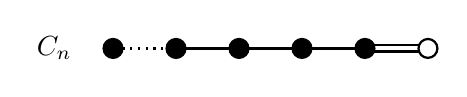
\begin{tikzpicture}[scale=.4]
    \draw (-1,0) node[anchor=east]  {$C_n$};
    \foreach \x in {0,...,4}
    \draw[xshift=\x cm,thick,fill=black] (\x cm,0) circle (.3cm);
    \draw[xshift=5 cm,thick] (5 cm, 0) circle (.3 cm);
    \draw[dotted,thick] (0.3 cm,0) -- +(1.4 cm,0);
    \foreach \y in {1.15,...,3.15}
    \draw[xshift=\y cm,thick] (\y cm,0) -- +(1.4 cm,0);
    \draw[thick] (8.3 cm, .1 cm) -- +(1.4 cm,0);
    \draw[thick] (8.3 cm, -.1 cm) -- +(1.4 cm,0);
  \end{tikzpicture}
}

\newcommand{\DynkinCab}{
  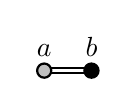
\begin{tikzpicture}[scale=.3]
    \draw (0,0.2) node[anchor=south] {$a$};
    \draw (2,0.2) node[anchor=south] {$b$};
    \foreach \x in {0}
    \draw[xshift=\x cm,thick,fill=lightgray] (\x cm,0) circle (.3cm);
    \foreach \x in {1}
    \draw[xshift=\x cm,thick,fill=black] (\x cm,0) circle (.3cm);
    \foreach \y in {0.15,...,0.15}
    \draw[xshift=\y cm,thick] (\y cm,+0.1 cm) -- +(1.4 cm,0);
    \foreach \y in {0.15,...,0.15}
    \draw[xshift=\y cm,thick] (\y cm,-0.1 cm) -- +(1.4 cm,0);
  \end{tikzpicture}
}

\newcommand{\DynkinCabc}{
  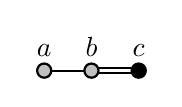
\begin{tikzpicture}[scale=.3]
    \draw (0,0.2) node[anchor=south] {$a$};
    \draw (2,0.2) node[anchor=south] {$b$};
    \draw (4,0.2) node[anchor=south] {$c$};
    \foreach \x in {0,1}
    \draw[xshift=\x cm,thick,fill=lightgray] (\x cm,0) circle (.3cm);
    \foreach \x in {2}
    \draw[xshift=\x cm,thick,fill=black] (\x cm,0) circle (.3cm);
    \foreach \y in {0.15,...,0.15}
    \draw[xshift=\y cm,thick] (\y cm,0) -- +(1.4 cm,0);
    \foreach \y in {1.15,...,1.15}
    \draw[xshift=\y cm,thick] (\y cm,+0.1 cm) -- +(1.4 cm,0);
    \foreach \y in {1.15,...,1.15}
    \draw[xshift=\y cm,thick] (\y cm,-0.1 cm) -- +(1.4 cm,0);
  \end{tikzpicture}
}


\newcommand{\DynkinDn}{
  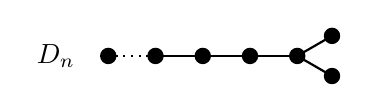
\begin{tikzpicture}[scale=.3]
    \draw (-1,0) node[anchor=east]  {$D_n$};
    \foreach \x in {0,...,4}
    \draw[xshift=\x cm,thick,fill=black] (\x cm,0) circle (.3cm);
    \draw[xshift=8 cm,thick,fill=black] (30: 17 mm) circle (.3cm);
    \draw[xshift=8 cm,thick,fill=black] (-30: 17 mm) circle (.3cm);
    \draw[dotted,thick] (0.3 cm,0) -- +(1.4 cm,0);
    \foreach \y in {1.15,...,3.15}
    \draw[xshift=\y cm,thick] (\y cm,0) -- +(1.4 cm,0);
    \draw[xshift=8 cm,thick] (30: 3 mm) -- (30: 14 mm);
    \draw[xshift=8 cm,thick] (-30: 3 mm) -- (-30: 14 mm);
  \end{tikzpicture}}

\newcommand{\DynkinGtwo}{
  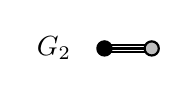
\begin{tikzpicture}[scale=.3]
    \draw (-1,0) node[anchor=east]  {$G_2$};
    \draw[thick,fill=black] (0 ,0) circle (.3 cm);
    \draw[thick,fill=lightgray] (2 cm,0) circle (.3 cm);
    \draw[thick] (30: 3mm) -- +(1.5 cm, 0);
    \draw[thick] (0: 3 mm) -- +(1.4 cm, 0);
    \draw[thick] (-30: 3 mm) -- +(1.5 cm, 0);
  \end{tikzpicture}}

\newcommand{\DynkinFfour}{
  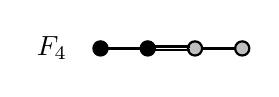
\begin{tikzpicture}[scale=.3]
    \draw (-3,0) node[anchor=east]  {$F_4$};
    \draw[thick,fill=black] (-2 cm ,0) circle (.3 cm);
    \draw[thick,fill=black] (0 ,0) circle (.3 cm);
    \draw[thick,fill=lightgray] (2 cm,0) circle (.3 cm);
    \draw[thick,fill=lightgray] (4 cm,0) circle (.3 cm);
    \draw[thick] (15: 3mm) -- +(1.5 cm, 0);
    \draw[xshift=-2 cm,thick] (0: 3 mm) -- +(1.4 cm, 0);
    \draw[thick] (-15: 3 mm) -- +(1.5 cm, 0);
    \draw[xshift=2 cm,thick] (0: 3 mm) -- +(1.4 cm, 0);
  \end{tikzpicture}}

\newcommand{\DynkinEsix}{
  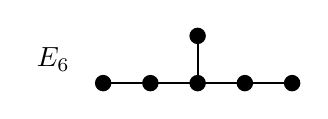
\begin{tikzpicture}[scale=.3]
    \draw (-1,1) node[anchor=east]  {$E_6$};
    \foreach \x in {0,...,4}
    \draw[thick,fill=black,xshift=\x cm] (\x cm,0) circle (3 mm);
    \foreach \y in {0,...,3}
    \draw[thick,xshift=\y cm] (\y cm,0) ++(.3 cm, 0) -- +(14 mm,0);
    \draw[thick,fill=black] (4 cm,2 cm) circle (3 mm);
    \draw[thick] (4 cm, 3mm) -- +(0, 1.4 cm);
  \end{tikzpicture}}

\newcommand{\DynkinEseven}{
  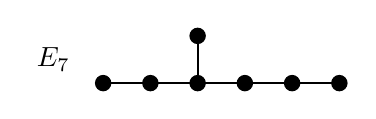
\begin{tikzpicture}[scale=.3]
    \draw (-1,1) node[anchor=east]  {$E_7$};
    \foreach \x in {0,...,5}
    \draw[thick,fill=black,xshift=\x cm] (\x cm,0) circle (3 mm);
    \foreach \y in {0,...,4}
    \draw[thick,xshift=\y cm] (\y cm,0) ++(.3 cm, 0) -- +(14 mm,0);
    \draw[thick,fill=black] (4 cm,2 cm) circle (3 mm);
    \draw[thick] (4 cm, 3mm) -- +(0, 1.4 cm);
  \end{tikzpicture}}

\newcommand{\DynkinEeight}{
  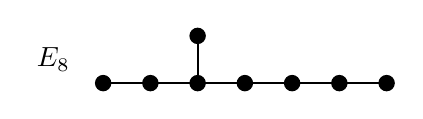
\begin{tikzpicture}[scale=.3]
    \draw (-1,1) node[anchor=east]  {$E_8$};
    \foreach \x in {0,...,6}
    \draw[thick,fill=black,xshift=\x cm] (\x cm,0) circle (3 mm);
    \foreach \y in {0,...,5}
    \draw[thick,xshift=\y cm] (\y cm,0) ++(.3 cm, 0) -- +(14 mm,0);
    \draw[thick,fill=black] (4 cm,2 cm) circle (3 mm);
    \draw[thick] (4 cm, 3mm) -- +(0, 1.4 cm);
  \end{tikzpicture}}




\title{Sketching Algebraic Groups}

%\author{Sijato Budotr}
\author{Simon Burton}

\date{\today}

\flushbottom

\begin{document}

\maketitle

%\begin{abstract}
%\end{abstract}

%\tableofcontents

%\doublespacing
%\onehalfspacing

\section{Representation theory of $S_n$}

% https://golem.ph.utexas.edu/category/2007/04/schur_functors.html#c008943
%    There are two Schur functors, corresponding to the partitions
%    (2) and (1,1); I’ll denote them by S2S^2 and S1,1S^{1,1}.
%    The definition (according to Fulton) is that S2(V)S^2(V)
%    is the quotient of V⊗2V^{\otimes 2} by the subspace spanned
%    by expressions of the form u⊗v−v⊗uu \otimes v - v \otimes
%    u; the definition of S1,1(V)S^{1,1}(V) is the quotient
%    of V⊗2V^{\otimes 2} by the subspace spanned by elements
%    of the forms u⊗uu \otimes u and u⊗v+v⊗uu \otimes v +
%    v \otimes u. It is easy enough to see how S2S^2 and S1,1S^{1,1}
%    should act on morphisms.
%    
%    Now, any construction involving quotients should have
%    a dual construction involving subspaces. So let S2(V)S_2(V)
%    be the kernel of V⊗2→S1,1(V)V^{\otimes 2} \to S^{1,1}(V)
%    and let S1,1(V)S_{1,1}(V) be the kernel of V⊗2→S2(V)V^{\otimes
%    2} \to S^2(V). S2S_2 and S1,1S_{1,1} are also functors
%    in a clear way.


We have the decomposition
$$
    V^{\tensor 2} \cong \yng(2)(V) \oplus \yng(1,1)(V)
$$
or, just counting dimensions:
\begin{center}
\begin{tabular}{cccc}
V  &    $V^{\otimes 2}$ &  $\yng(2)(V)$  &  $\yng(1,1)(V)$   \\
    \hline
0&    0  &  0   &  0   \\
1&    1  &  1   &  0   \\
2&    4  &  3   &  1   \\
3&    9  &  6   &  3   \\
4&    16  &  10   &  6   \\
... &  &     &     \\
\end{tabular}
\end{center}

Going to a third tensor power, we get
$$
    V^{\tensor 3} \cong \yng(3)(V) \oplus 
        2\cdot \yng(1,2)(V) \oplus \yng(1,1,1)(V).
$$
In general these tensor powers $V^{\tensor n}$ decompose as
a sum over Young diagrams $\lambda$ with number of boxes $|\lambda|=n$,
and with multiplicity $m_\lambda$:
$$
V^{\tensor n} \cong \bigoplus_{|\lambda|=n}
    m_\lambda\cdot \lambda(V).
$$

A categorified binomial theorem (\cite{Brandenburg2014} Lemma 3.2.1).
Given finite dimensional vector spaces $V,W$ and $n\in\Natural$,
$$
    (V\oplus W)^{\tensor n} \cong 
        \bigoplus_{m=0}^n
        {n\choose m}\cdot
        V^{\tensor m}\tensor W^{\tensor (n-m)}.
$$
Now we combine this binomial theorem with the
observations above, any Young diagram $\lambda$ with $n$ boxes
we have a map:
$$
    \lambda(V\oplus W) \to 
        \bigoplus_{m=0}^n
        {n\choose m}\cdot
        V^{\tensor m}\tensor W^{\tensor (n-m)}.
$$
So there should be a binomial formula for each Young diagram.
Here are two examples:
\begin{align*}
\yng(1,2)(V\oplus W) 
\cong\ \ \ \   & \yng(1,2)(V)\tensor\phi(W) \\
\oplus\ & \yng(2)(V)  \tensor\yng(1)(W)  \\
\oplus\ & \yng(1,1)(V)  \tensor\yng(1)(W)  \\
\oplus\ & \yng(1)(V)  \tensor\yng(2)(W)  \\
\oplus\ & \yng(1)(V)  \tensor\yng(1,1)(W)  \\
\oplus\ & \phi(V)  \tensor\yng(1,2)(W) .
\end{align*}
The empty Young diagram is $\phi$ and $\phi(V)\cong \Complex.$
Another example:
\begin{align*}
\yng(2,2)(V\oplus W) 
\cong\ \ \ \   & \yng(2,2)(V)\tensor\phi(W) \\
\oplus\ & \yng(1,2)(V)  \tensor\yng(1)(W)  \\
\oplus\ & \yng(2)(V)  \tensor\yng(2)(W)  \\
\oplus\ & \yng(1,1)(V)  \tensor\yng(1,1)(W)  \\
\oplus\ & \yng(1)(V)  \tensor\yng(1,2)(W)  \\
\oplus\ & \phi(V)  \tensor\yng(2,2)(W) .
\end{align*}

\section{Algebraic groups}

The slick definition of an algebraic group is
a group object in the category of affine schemes.
Instead of worrying about what is the category of
affine schemes, we just define this to be the opposite
of the category of commutative rings, $\CRing$.

\section{Representation theory of GL(n)}

We are considering algebraic groups over the field of
complex numbers, and the monoidal category of representations of 
these groups.

\subsection{GL(1)}

TODO

\subsection{GL(2)}

This pair of short exact sequences are key
to understanding the following:
\[
\begin{tikzcd}
    &  
    \SL(2) \arrow[rightarrowtail]{d}\arrow[two heads]{dr}{\mathrm{2-to-1}} &  \\
    \GL(1) \arrow[rightarrowtail]{r}{\mathrm{diag}} 
           \arrow[two heads]{dr}[below,left]{\mathrm{2-to-1\ }}  &  
    \GL(2) \arrow[two heads]{r}\arrow[two heads]{d}{\mathrm{det}}  &  \PGL(2)     \\
    &  \GL(1)             &     \\
\end{tikzcd}
\]


We label the irreducible represenations of SL(2) by
Young diagrams with one row:
\begin{center}
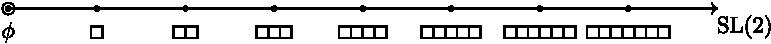
\includegraphics[]{images/sl2.pdf}
\end{center}

Within these, we have a subcategory of represenations of PGL(2):
\begin{center}
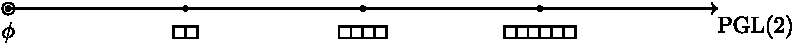
\includegraphics[]{images/pgl2.pdf}
\end{center}

The irreducible represenations of GL(2) look like this:
\begin{center}
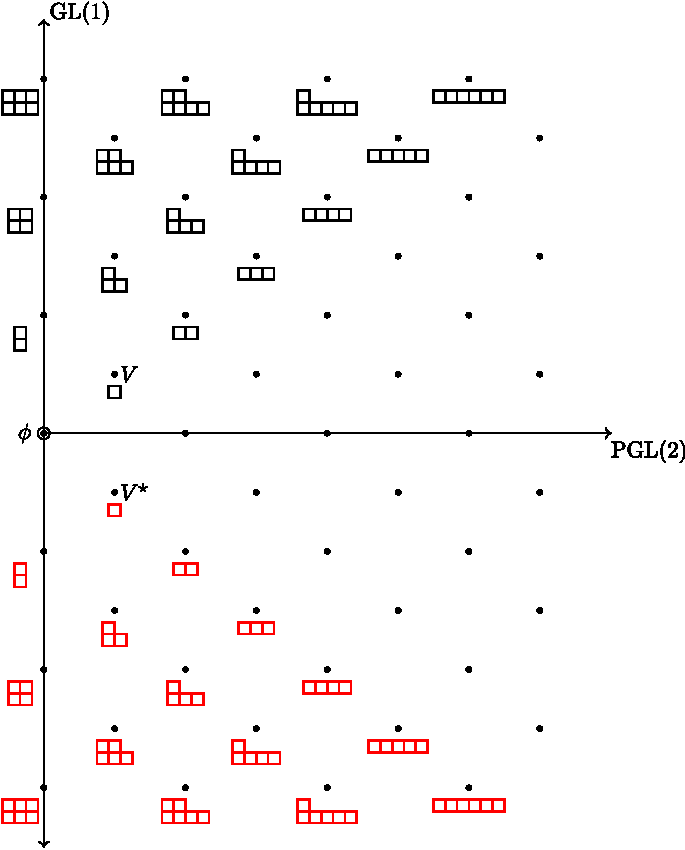
\includegraphics[scale=0.8]{images/gl2.pdf}
\end{center}
Where we have labelled the tautological (natural) represenation as $V$
and its dual as $V^{\star}.$

\subsection{GL(3)}

\[
\begin{tikzcd}
    &  
    \SL(3) \arrow[rightarrowtail]{d}\arrow[two heads]{dr}{\mathrm{3-to-1}} &  \\
    \GL(1) \arrow[rightarrowtail]{r}{\mathrm{diag}} 
           \arrow[two heads]{dr}[below,left]{\mathrm{3-to-1\ }}  &  
    \GL(3) \arrow[two heads]{r}\arrow[two heads]{d}{\mathrm{det}}  &  \PGL(3)     \\
    &  \GL(1)             &     \\
\end{tikzcd}
\]

We start with a picture of the $\SL(3)$ kaleidoscope:
\begin{center}
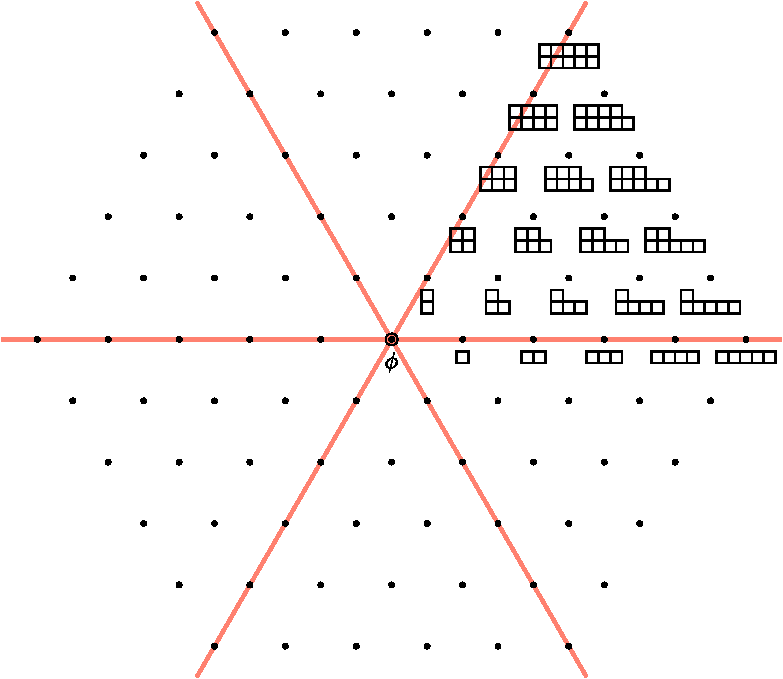
\includegraphics[scale=0.8]{images/sl3.pdf}
\end{center}

The epimorphism SL(3)$\to$PGL(3) is a 3-to-1 map,
and so we find the irreps of PGL(3) as an index 3 
sublattice of the SL(3) kaleidoscope:
\begin{center}
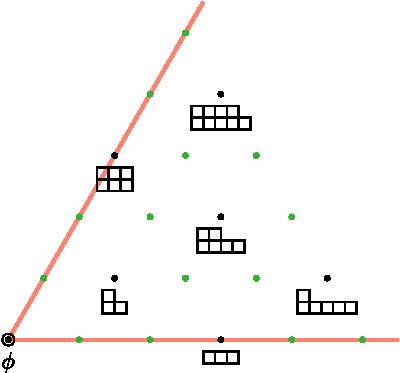
\includegraphics[scale=0.8]{images/pgl3.pdf}
\end{center}

The positive levels of $\GL(3)$:
\begin{center}
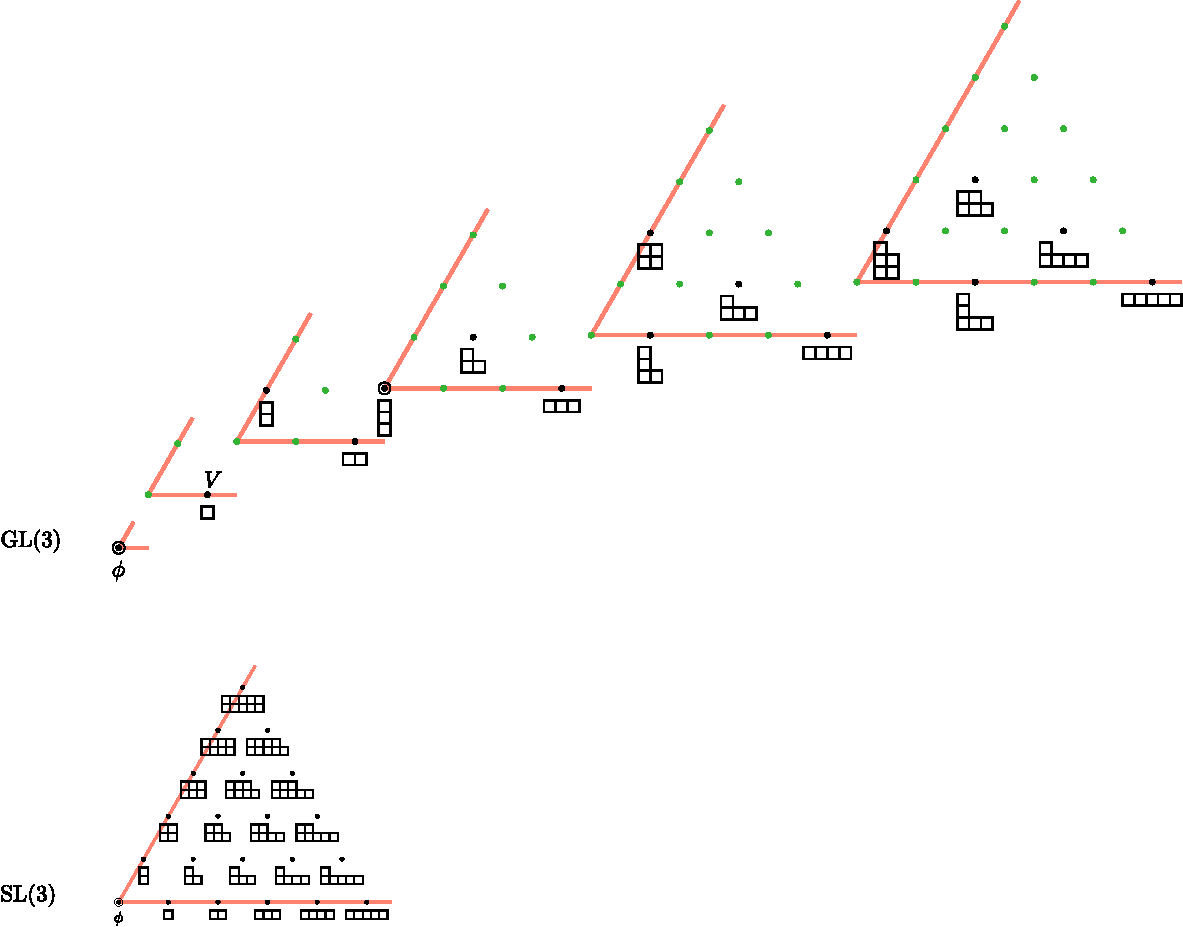
\includegraphics[scale=0.6]{images/gl3.pdf}
\end{center}

\section{Dimension of irreducibles}

%\begin{center}
%\begin{tabular}{ccc}
%hi & there & xyz \\
%hi & there & xyz \\
%hi & there & xyz \\
%\end{tabular}
%\end{center}

Here we record some observational mathematics, ie. numerology,
got by torturing sage python and eyeballing the results.
We try to be brief, before someone calls the mathematics police on us.

\subsection{The $A$ series}


The $A_n$ series Dynkin diagram has $n$ nodes:
$$ \DynkinAn $$
In the following table we have labelled
each node in the Dynkin diagram with a natural number,
and use these numbers to label the complex irreducible
representations of $\SL(n+1,\Complex)$.
The dimension of each of these representations
can be written as a multivariate polynomial in the labels of degree 
$n(n+1)/2$ which has linear factors of a nice form.
Each of these factors involves labels from a contiguous subset on
the labelled Dynkin diagram.

$$
\begin{array}{c|c|rl}
\text{Lie group} & \text{Dynkin diagram} & \text{dimension} & \\
\hline
\SL(2,\Complex)           & \DynkinAa   & A_1(a) =& a+1 \\
\SL(3,\Complex)           & \DynkinAab  & A_2(a,b) =& (a+1)(b+1)(a+b+2)/2 \\
\SL(4,\Complex)           & \DynkinAabc   & A_3(a,b,c) =& (a+1)(b+1)(c+1) \\
 & & &\ \ (a+b+2)(b+c+2)(a+b+c+3)/12 \\
\SL(5,\Complex)           & \DynkinAabcd  & A_4(a,b,c,d) =& (a+1)(b+1)(c+1)(d+1) \\
 & & &\ \ (a+b+2)(b+c+2)(c+d+2) \\
 & & &\ \ (a+b+c+3)(b+c+d+3) \\
    & & & \ \ (a+b+c+d+4)/288 \\
\end{array}
$$

Evidently there is a nice recurrence relation,
$$
    A_n(x_1,...,x_n) = A_{n-1}(x_1,...,x_{n-1})
    (x_n + 1)
    (x_{n-1} + x_n + 2)
    ...
    (x_1 + ... + x_n + n) 
    / n!
$$

\subsection{The $B$ series}

The Lie group corresponding to $B_n$ is $\SO(2n+1).$
The dimension counting polynomial $B_n(x_1,...,x_n)$ is
of degree $n^2.$

$$
\begin{array}{c|c|rl}
\text{Lie group} & \text{Dynkin diagram} & \text{dimension} & \\
\hline
\SO(5,\Complex) & \DynkinBab  & B_2(a,b) =& (a+1)(2b+1)(2a+2b+3)(2a+4b+4)/12 \\
\SO(7,\Complex) & \DynkinBabc & B_3(a,b,c) =& (a+1)(b+1)(2c+1) \\
                             & & &\ \ (a+b+2)(b+2c+2)(2b+2c+3) \\
                             & & &\ \ (a+b+2c+3)(a+2b+2c+4) \\
            & & &\ \ (2a+2b+2c+5)/720 \\
\end{array}
$$


\subsection{The $C$ series}

The Lie group corresponding to $C_n$ is $\Sp(2n).$
The dimension counting polynomial $C_n(x_1,...,x_n)$ is
of degree $n^2.$

$$
\begin{array}{c|c|rl}
\text{Lie group} & \text{Dynkin diagram} & \text{dimension} & \\
\hline
\Sp(4,\Complex) & \DynkinCab  & C_2(a,b) =& (a+1)(b+1)(a+b+2)(a+2b+3)/6 \\
\Sp(6,\Complex) & \DynkinCabc & C_3(a,b,c) =& (a+1)(b+1)(c+1) \\
                             & & &\ \ (a+b+2)(b+c+2)(b+2c+3)\\
                             & & &\ \ (a+b+c+3)(a+b+2c+4)\\
            & & &\ \ (a+2b+2c+5)/720 \\
\end{array}
$$

In general, we see that $C_n(x_1,...,x_n)$ has factor $A_n(x_1,...,x_n)$,
which accounts for $n(n+1)/2$ linear factors, with $n(n-1)/2$ linear
factors remaining to add up to the total of $n^2$.
For the next polynomial,
\begin{align*}
C_4(a, b, c, d) =& A_4(a, b, c, d) \\
    &\ \  (a+b+c+2d+5) \\
    &\ \  (a+b+2c+2d+6)(b+c+2d+4) \\
    &\ \  (a+2b+2c+2d+7)(b+2c+2d+5)(c+2d+3)/(5\times 6\times 4\times 7\times 5\times 3).
\end{align*}

\subsection{The $D$ series}

The Lie group corresponding to $D_n$ is $\SO(2n).$
$$
\DynkinDn
$$

So far we have only found the following polynomial of degree 12:
$$
D_4(a, a, a, a) = (a+1)^6(2a+1)(3a+2)(3a+1)(5a+3)^2(7a+5).
$$

\subsection{$G_2$}

The Dynkin diagram for $G_2$ is
$$
\DynkinGtwo
$$

The dimension polynomial is:
\begin{align*}
G_2(a, b) =& \frac{1}{120} (1+a)(1+b)(2+a+b)(3+a+2b)(4+a+3b)(5+2a+3b).
\end{align*}

\subsection{The other exceptionals}

We still have remaining: % $G_2, F_4, E_6, E_7, E_8.$

$$
\DynkinFfour
$$

$$
\DynkinEsix
$$

$$
\DynkinEseven
$$

$$
\DynkinEeight
$$

% ---------------------------------------------------------

\section{Notes}

References: 
\cite{Fulton2013}
\cite{Goodman2009}
\cite{Kraft2000}
\cite{Mukai2003}
\cite{Procesi2007}
\cite{Bump2004}
\cite{Miller2004}


\bibliography{refs2}{}
\bibliographystyle{abbrv}

\end{document}
